%%%%%%%%%%%%%%%%%%%%%%%%%%%%%%%%%%%%%%%%%%%%%%%%%%%%%%%%%%%%%%%%%%%%%%
% How to use writeLaTeX: 
%
% You edit the source code here on the left, and the preview on the
% right shows you the result within a few seconds.
%
% Bookmark this page and share the URL with your co-authors. They can
% edit at the same time!
%
% You can upload figures, bibliographies, custom classes and
% styles using the files menu.
%
%%%%%%%%%%%%%%%%%%%%%%%%%%%%%%%%%%%%%%%%%%%%%%%%%%%%%%%%%%%%%%%%%%%%%%

\documentclass[12pt]{article}
\usepackage[pdftex]{hyperref}
\usepackage[table,xcdraw]{xcolor}


\usepackage{sbc-template}
\usepackage{listings}

\usepackage{graphicx,url}

%\usepackage[brazil]{babel}   
\usepackage[utf8]{inputenc}  
\usepackage{float}
\sloppy

\title{Pré-projeto: Controlador de repedidor de sinal wi-fi acionado via telegram}

\author{João Vitor Moreira Duarte }


\address{Instituto de Federal de Educação e Tecnologia -- Campús do Maracanaú
  (IFCE)\\
  Av. Parque Central, 1315 - Distrito Industrial I, Maracanaú - CE, 61939-140
  \email{joao.vitor.moreira08@aluno.ifce.edu.br}
}

\begin{document}

\maketitle
\begin{resumo}
  Esse documento tem como proposta apresentar a ideia inicial para o trabalho final da cadeira de microcontroladores
  ministrada pelo professor, Sandro Cesar Silveira Juca no Instituto de Federal de Educação e Tecnologia(IFCE) campus Maracanaú.
  A ideia sugerida é utilizar o microcontrolador ESP32, para repetir o sinal de uma rede wi-fi e controlar o acionamento
  do repedidor por meio de um bot do telegram com possíveis funcionalidades para monitorar o uso da rede.
\end{resumo}


\section{Introdução}
Segundo \cite{ALMEIDA} a automação residencial ainda possui um alto custo para o
grupo ao qual se destina. Tendo em vista que nem todos tem acesso a grandes orçamentos para tentar automatizar sua residencia,
é de grande importância que seja possível criar soluções baixo custo quando pensamos em automatizar alguma parte do dia a dia dentro de uma residencia.

Dessa forma projetos como repetidores de wi-fi simples e de custo baixo são uma boa porta de entrada para uma casa mais automatizada,
assim utilizando o microcontrolador ESP32 que tem um custo relativamente baixo comparado com os repetidores de sinal que vemos hoje no mercado
é possível deixar uma residencia mais \emph{smart}.

\section{Fundamentação Teórica}
Para esse projeto foi levado em consideração a assediabilidade para reprodução, dessa forma o projeto visa utilizar somente de softwares gratuitos e materiais de baixo custo.
Com isso, usaremos somente o microcontrolador ESP32 pelo seu preço acessível e sua capacidade de conectar-se a uma rede sem fio, para fazer a comunicação entre usuário e
controlador sera feito uso do software gratuito, telegram e sua funcionalidade de criar bots dentro do aplicativo, estes irão acionar o nosso esp. E para ambiente de desenvolvimento,
sera utilizado o Arduino IDE, que é uma ferramenta para programar placas como o ESP, Arduino e raspberry's.

\subsection{ESP32}
É um pequeno microcontrolador que tem suporte tanto para Wi-fi e Bluetooth. Seu pequeno tamanho e a sua grande eficiência fazem com que este dispositivo
destaca-se dentre tantos outros.

\begin{figure}[ht]
  \centering
  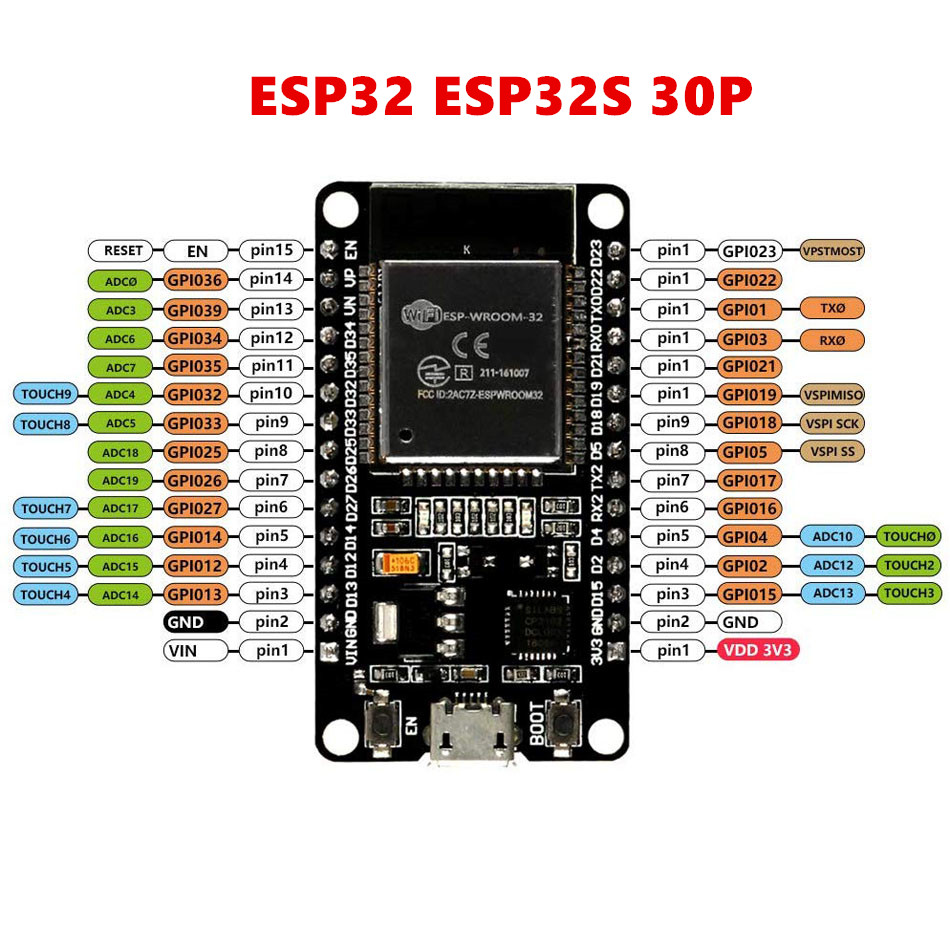
\includegraphics[width=.35\textwidth]{Images/ESP32.jpg}
  \caption{ESP32}
  \label{fig:exampleESP32}
\end{figure}

\subsection{ArduinoIDE}
É uma aplicação de plataforma cruzada, escrito em funções de C e C ++. É usado para escrever e fazer upload de
programas em placas compatíveis com Arduino, mas também, com a ajuda de núcleos de terceiros, outras placas de
desenvolvimento de fornecedores.

Para exportar o código para o nosso ESP32 foi adicionado a placa dentro da IDE para que o fosse reconhecido corretamente.

\begin{figure}[ht]
  \centering
  
\includegraphics[width=.25\textwidth]{Images/arduinoIDELogo.png}
  \caption{Logo de ArduinoIDE}
  \label{fig:exampleArduinoIDE}
\end{figure}


\subsection{Telegram e Bot}
O Telegram é um aplicativo gratuito de mensagens que pode ser acessado tanto do \emph{smartphone} quanto pela \emph{web}
usaremos ele para gerenciar o controle do nosso repedidor.
O telegram tem como diferencial a possibilidade de criar bots usando uma ferramenta apelidada de \emph{botfather},
bots criados por ele podem receber comandos para executar algumas ações e é por meio de um bot criado por ele que faremos a comunicação com
nosso repetidor.

\begin{figure}[ht]
  \centering
  
\includegraphics[width=.25\textwidth]{Images/header.png}
  \caption{Logo de ArduinoIDE e botfather}
  \label{fig:exampleTelegram}
\end{figure}

\section{Metodologia}
Usando as ferramentas apresentadas, é proposto criar um bot por meio do telegram, que se comunique com o microcontrolador para acionar a repetição de sinal
com as instruções passadas para o esp32 por meio do ArduinoIDE incluindo respostas para informar status do aparelho para o usuário.

\section{Cronograma}

\begin{table}[hb]
  \centering
  \begin{tabular}{|l|c|c|c|}
    \hline
    \rowcolor[HTML]{9B9B9B}
    Atividade                    & out & nov & dez \\ \hline
    \rowcolor[HTML]{C0C0C0}
    Construção do bot e codigo   & X   &     &     \\ \hline
    \rowcolor[HTML]{C0C0C0}
    Integração do bot com codigo & X   & X   &     \\ \hline
    \rowcolor[HTML]{C0C0C0}
    Testes do repetidor          &     &     & X   \\ \hline
  \end{tabular}
\end{table}
\bibliographystyle{sbc}
\bibliography{sbc-template}
\end{document}
